%!TEX root = notes.tex

\section*{Exercises}
\begin{problem}\label{problem:maxima}
Develop similar statements as in Definition \ref{def:localminimum}, Theorems \ref{theorem:localminimum}, \ref{theorem:2DTforLEV} and \ref{theorem:MaxMinCompact}, but for \emph{local} and \emph{global maxima}.
\end{problem}

\begin{problem}[Domains]
Find and sketch the domain of the following functions.
\begin{enumerate}
	\item $f(x,y) = \sqrt{y-x-2}$
	\item $f(x,y) = \log \big( x^2+y^2-4 \big)$
	\item $f(x,y) = \frac{(x-1)(y+2)}{(y-x)(y-x^3)}$
	\item $f(x,y) = \log (xy+x-y-1)$
\end{enumerate}
\end{problem}

\begin{problem}[Contour plots]
Find and sketch the level lines $f(x,y)=c$ on the same set of coordinate axes for the given values of $c$.
\begin{enumerate}
	\item $f(x,y) = x+y-1$, $c \in \{ -3, -2, -1, 0, 1, 2, 3\}$.
	\item $f(x,y) = x^2+y^2$, $c \in \{ 0, 1, 4, 9, 16, 25 \}$.
	\item $f(x,y) = xy$, $c \in \{ -9, -4, -1, 0, 1, 4, 9 \}$
\end{enumerate}
\end{problem}

\begin{problem}\label{problem:countours}
Use a Computer Algebra System of your choice to produce contour plots of the given functions on the given domains.
\begin{enumerate}
	\item $f(x,y) = (\cos x)(\cos y) e^{-\sqrt{x^2+y^2}/4}$ on $[-2\pi, 2\pi]\times [-2\pi, 2\pi]$.
	\item $g(x,y) = \dfrac{xy(x^2-y^2)}{x^2+y^2}$ on $[-1,1] \times [-1,1]$
	\item $h(x,y) = y^2 - y^4 -x^2$ on $[-1,1]\times[-1,1]$
	\item $k(x,y) = e^{-y}\cos x$ on $[-2\pi, 2\pi]\times[-2,0]$
\end{enumerate}
\begin{figure}[ht!]
\begin{tabular}{cc}
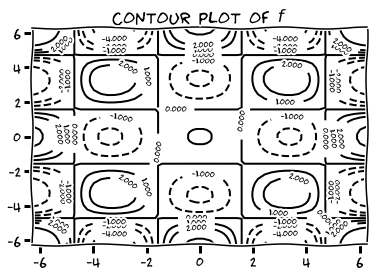
\includegraphics[width=0.5\linewidth]{contourf.png} &
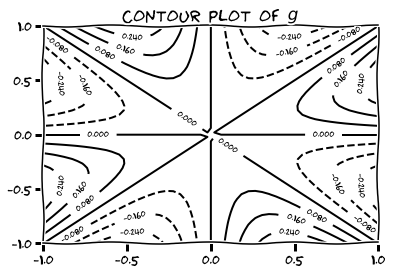
\includegraphics[width=0.5\linewidth]{contourg.png} \\
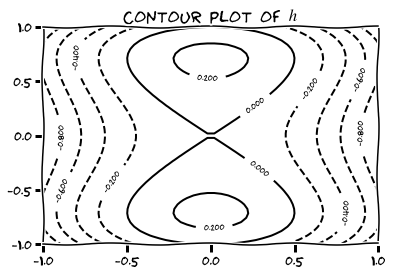
\includegraphics[width=0.5\linewidth]{contourh.png} &
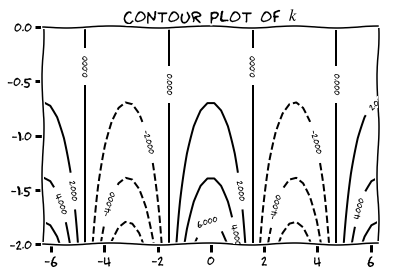
\includegraphics[width=0.5\linewidth]{contourk.png} 
\end{tabular}
\caption{Contour plots for problem \ref{problem:countours}}
\end{figure}
\end{problem}

\begin{problem} % example 2, p.858 in Thomas' Calculus
Find the points of the hyperbolic cylinder $x^2=z^2-1=0$ in $\field{R}^3$ that are closest to the origin.
\end{problem}

